\section{Beschreibung von Signalen im Zeitbereich}

\textbf{Hinweis:} Sofern nichts anderes angegeben sind Signale $x(t)$ im Zeitbereich reelle Signale!


\subsection[Linearer Mittelwert]{Linearer Mittelwert $\bm{X_0 = X_m = \overline{X}}$}{5}

Der lineare Mittelwert des \textbf{reellen Signals $\bm{x(t)}$} ist definiert als:

\vspace{-0.2cm}

\begin{minipage}[t]{0.48\columnwidth}
    \begin{center}
        $$ \boxed{ X_0 = \frac{1}{T} \int\limits_{-T/2}^{T/2} x(t) \, \diff t } $$
        Klasse 2a
    \end{center}
\end{minipage}
\hfill
\begin{minipage}[t]{0.48\columnwidth}
    \begin{center}
        $$ \boxed{ X_0 = \lim\limits_{T \to \infty} \frac{1}{T} \int\limits_{-T/2}^{T/2} x(t) \, \diff t } $$
        Klasse 2b
    \end{center}
\end{minipage}


\subsection[Quadratischer Mittelwert]{Quadratischer Mittelwert $\bm{X^2}$}{6}

Der quadratische Mittelwert von \textbf{reellen, periodischen Leistungssignalen} (Klasse 2a) ist ein \textbf{Mass für die Leistung}
und ist definiert als:

$$ \boxed{ X^2 = \frac{1}{T} \int\limits_{-T/2}^{T/2} x^2(t) \, \diff t } $$

Es gilt stets: $X^2 \geq 0$


\subsection[Effektivwert (RMS)]{Effektivwert $\bm{X_{\rm eff}}$ (RMS)}

$$ \boxed{ X_{\rm eff} = \sqrt{X^2} } $$

Es gilt: $X_{\rm eff} > X_m$


\subsection[Mittelwert n. Ordnung]{Mittelwert $\bm{n.}$ Ordnung}{6}

Die Mittelwerte $n.$ Ordnung von \textbf{reellen, periodischen Leistungssignalen} (Klasse 2a) sind definiert als:

$$ \boxed{ X^n = \frac{1}{T} \int\limits_{-T/2}^{T/2} x^n(t) \, \diff t } $$


\subsection[Varianz]{Varianz $\bm{\Var(x) = \sigma^2}$}{7}

Die Varianz (1. zentrales Moment) ist der quadratische Mittelwert des rellen Signals $x(t)$ um $X_0$ 

$$ \boxed{ \Var(x) = \sigma^2 = \frac{1}{T} \int\limits_{-T/2}^{T/2} \big( x(t) - X_0 \big)^2  \, \diff t } $$

Es gilt stets: $\Var(x) \geq 0$


\subsection[Standardabweichung]{Standardabweichung $\bm{\sigma}$}

Wurzel der Varianz

$$ \boxed{ \sigma = \sqrt{\Var(x)} } $$


\subsection{Zusammenhänge}

Die Varianz $\Var(x)$, der quadratische Mittelwert $X^2$ und der lineare Mittelwert $X_0$ hängen folgendermassen zusammen:

$$ \boxed{ \Var(x) = \sigma^2 = X^2 - (X_0)^2 } $$

Für reelle Signale gilt:

$$ \boxed{ X^2  = \Var(x) + X_0^2 = \vert X \vert^2 = \Var(\vert x \vert) + \vert X_0 \vert ^2} $$


\subsection{Tipps und Tricks zur Mittelwert-Berechnung}

\begin{itemize}
	\item Skizzen machen und grafisch überlegen
	\item Integralgrenzen geschickt wählen (z.B. $0 \ldots T$ oder 2 Mal Integral mit Grenzen $0 \ldots \frac{T}{2}$)
\end{itemize}


\subsection{Übersicht wichtige Funktions-Mittelwerte}

\textbf{Hinweis:} Die Amplitude eines Signals wird als $A$ bezeichnet 

\begin{center}
    \renewcommand{\arraystretch}{1.6}
    \begin{tabular}{| l | c | c | c |}
        \hline
        \textbf{Signal}         & $\bm{X_0}$                    & $\bm{X^2}$        & $\bm{X_{\rm eff}}$                \\
        \hline
        $\sin(t)$               & $0$                           & $\frac{1}{2}$     & $\frac{\sqrt{2}}{2}$              \\
        \hline
        $\cos(t)$               & $0$                           & $\frac{1}{2}$     & $\frac{\sqrt{2}}{2}$              \\
        \hline
        $A \cdot \sin(t)$       & $0$                           & $\frac{A^2}{2}$   & $A \cdot \frac{\sqrt{2}}{2}$      \\
        \hline
        $A \cdot \cos(t)$       & $0$                           & $\frac{A^2}{2}$   & $A \cdot \frac{\sqrt{2}}{2}$      \\
        \hline
        $| A \cdot \sin(t) |$   & $| A | \cdot \frac{2}{\pi}$   & $\frac{A^2}{2}$   & $A \cdot \frac{\sqrt{2}}{2}$      \\
        \hline
        $| A \cdot \cos(t) |$   & $ | A | \cdot \frac{2}{\pi}$  & $\frac{A^2}{2}$   & $A \cdot \frac{\sqrt{2}}{2}$      \\
        \hline
        Dreieck \& Sägezahn     & $0$                           & $\frac{A^2}{3}$   &  $ A \cdot \frac{\sqrt{3}}{3}$    \\ 
        \hline
    \end{tabular}
    \renewcommand{\arraystretch}{1}
\end{center}

\textbf{Allfällige DC-Anteile der Signale ändern die Werte entsprechend!}


\subsection{Autokorrelationsfunktion (AKF)}{8-11}

Die AKF ist ein Mass für die innere Kohärenz (Ähnlichkeit)eines Signals. Sie ist eine Erweiterung des quadratischen Mittelwerts.
($\varphi_{xx}(0) = X^2$)


\subsubsection{AKF für reelle, periodische Leistungssignale (Klasse 2a)}

\vspace{-0.2cm}

$$ \boxed{  \varphi_{xx}(\tau) = \frac{1}{T} \int\limits_{-T/2}^{T/2} x(t) \, x(t-\tau) \, \diff t 
    = \frac{1}{T} \int\limits_{-T/2}^{T/2} x(t+\tau) \,x(t) \, \diff t = \varphi_{xx}(-\tau) } $$

\begin{center}
    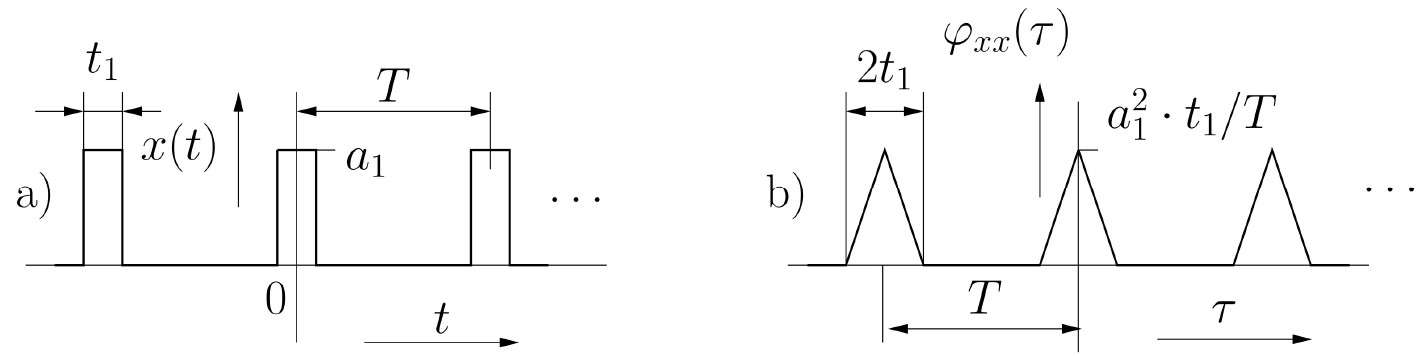
\includegraphics[width=0.8\columnwidth]{images/beispiel_AKF.jpg}
\end{center}


\subsubsection{AKF für stochastische Leistungssignale (Klasse 2b)}

\vspace{-0.2cm}

$$ \boxed{ \varphi_{xx}(\tau) = \frac{1}{T} \lim\limits_{T \to \infty} \int\limits_{-T/2}^{T/2} x(t) \, x(t-\tau) \, \diff t 
    = \frac{1}{T} \lim\limits_{T \to \infty}  \int\limits_{-T/2}^{T/2} x(t+\tau) \,x(t) \, \diff t = \varphi_{xx}(-\tau) } $$


\subsubsection{AKF für Energiesignale (Klasse 1)}

\vspace{-0.2cm}

$$ \boxed{ \varphi_{xx}(\tau) = \lim\limits_{T \to \infty}  \int\limits_{-T/2}^{T/2} x(t) \, x(t-\tau) \, \diff t 
    =  \lim\limits_{T \to \infty}  \int\limits_{-T/2}^{T/2} x(t+\tau) \,x(t) \, \diff t = \varphi_{xx}(-\tau) } $$


\subsubsection{Eigenschaften der Autokorrelationsfunktion (AKF)}

\begin{itemize}
    \setlength\itemsep{5pt}
    \item $\varphi_{xx}(0) = X^2 = (X_0)^2 + \sigma^2 $ \textrightarrow\ Quadratischer Mittelwert (Definition)
    \item $\varphi_{xx}(\tau) = \varphi_{xx}(\tau \pm n \cdot T)$ mit $n \in \mathbb{N}$ \\
        d.h. die AKF ist periodisch mit der gleichen Periode $T$ wie das Signal $x(t)$ 
    \item $\varphi_{xx}(\tau) = \varphi_{xx}(-\tau)$ d.h. AKF ist \textbf{gerade Funktion}
    \item $\varphi_{xx}(0) \geq \vert \varphi_{xx}(\tau) \vert$ , d.h. AKF am grössten bei vollständiger Deckung
    \item $\varphi_{xx}(\tau) \geq (X_0)^2 - \sigma^2$ 
\end{itemize}


\subsection{Kreuzkorrelationsfunktion (KKF)}{11-13}

Die KKF ist ein Mass für die \textbf{Ähnlichkeit von zwei verschiedenen} Signalen. \\
\textbf{Grafisch:} Signal $x_2$ über $x_1$ 'schieben'

\vspace{0.2cm}

\crd{\textbf{Die KKF von 2 Signalen mit verschiedenen Perioden ist immer 0} }


\subsubsection{KKF für reelle, periodeische Leistungssignale (Klasse 2a)}

$$ \boxed{ \varphi_{x_1 x_2}(\tau) = \frac{1}{T} \int\limits_{-T/2}^{T/2} x_1(t) \, x_2(t-\tau) \, \diff t 
    = \frac{1}{T} \int\limits_{-T/2}^{T/2} x_1(t+\tau) \, x_2(t) \, \diff t } $$

\begin{center}
    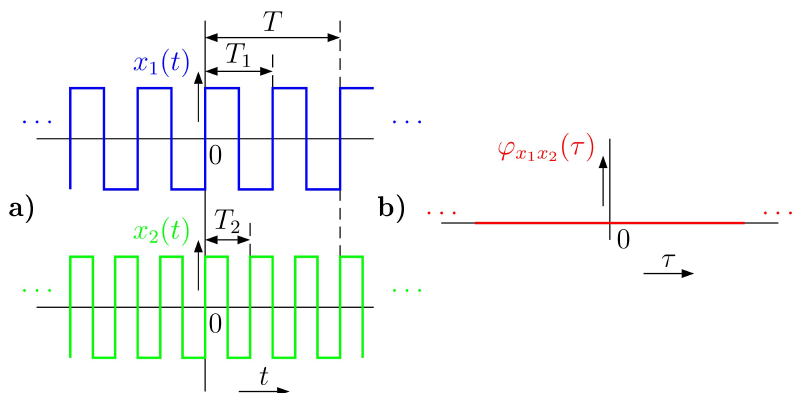
\includegraphics[width=0.7\columnwidth]{images/beispiel_KKF.png}
\end{center}


\subsubsection{KKF für stochastische Leistungssignale (Klasse 2b)}


$$ \boxed{ \varphi_{x_1 x_2}(\tau) = \lim\limits_{T \to \infty} \frac{1}{T} \int\limits_{-T/2}^{T/2} x_1(t) \, x_2(t-\tau) \, \diff t
    = \lim\limits_{T \to \infty}  \frac{1}{T} \int\limits_{-T/2}^{T/2} x_1(t+\tau) \, x_2(t) \, \diff t } $$


\subsubsection{KKF für Energiesignale (Klasse 1)}

$$ \boxed{ \varphi_{x_1 x_2}(\tau) = \lim\limits_{T \to \infty} \int\limits_{-T/2}^{T/2} x_1(t) \, x_2(t-\tau) \, \\diff t 
    = \lim\limits_{T \to \infty}  \int\limits_{-T/2}^{T/2} x_1(t+\tau) \, x_2(t) \, \diff t } $$


\subsection{Faltung}{14}

\vspace{-0.2cm}

$$ \boxed{ y(t) = x_1(t) * x_2(t) = (x_1 * x_2)(t) = \int\limits_{-\infty}^{\infty} x_1(\tau) \cdot x_2(t - \tau) \; \diff \tau } $$ 


\subsubsection{Grafische Faltung}

\textbf{Grafisch:} Signal $x_2$ an $y$-Achse spiegeln und \textbf{gespiegeltes} Signal über $x_1$ 'schieben' \\
(oder umgekehrt)

\vspace{0.2cm}

\begin{tabular}{ll}
    Startpunkt: & 'Addition vom Start der beiden Supports'                              \\
    Endpunkt: 	& 'Addition vom Ende der beiden Supports'                               \\
    Maximum:	& Wenn Überlappung beider Signale am grössten                           \\
                & \textrightarrow\ nach Anzahl geschobenen Zeitschritte                 \\
    Fläche 		& Die Fläche des Faltungsprodukts entspricht der Fläche unter $x_1$ mal \\
                & der Fläche unter $x_2$         
\end{tabular}


\subsubsection{Eigenschaften des Faltungsprodukts}

\renewcommand{\arraystretch}{1.3}
\begin{tabular}{ll}
    kommutativ:     & $f * g = g * f$                   \\
    assoziativ:     & $f * (g * h) = (f * g) * h$       \\
    distributiv:    & $f * (g + h) = f * g + f * h $
\end{tabular}
\renewcommand{\arraystretch}{1}


\subsection{Komplexe Frequenzen}{15-17}

\begin{center}
    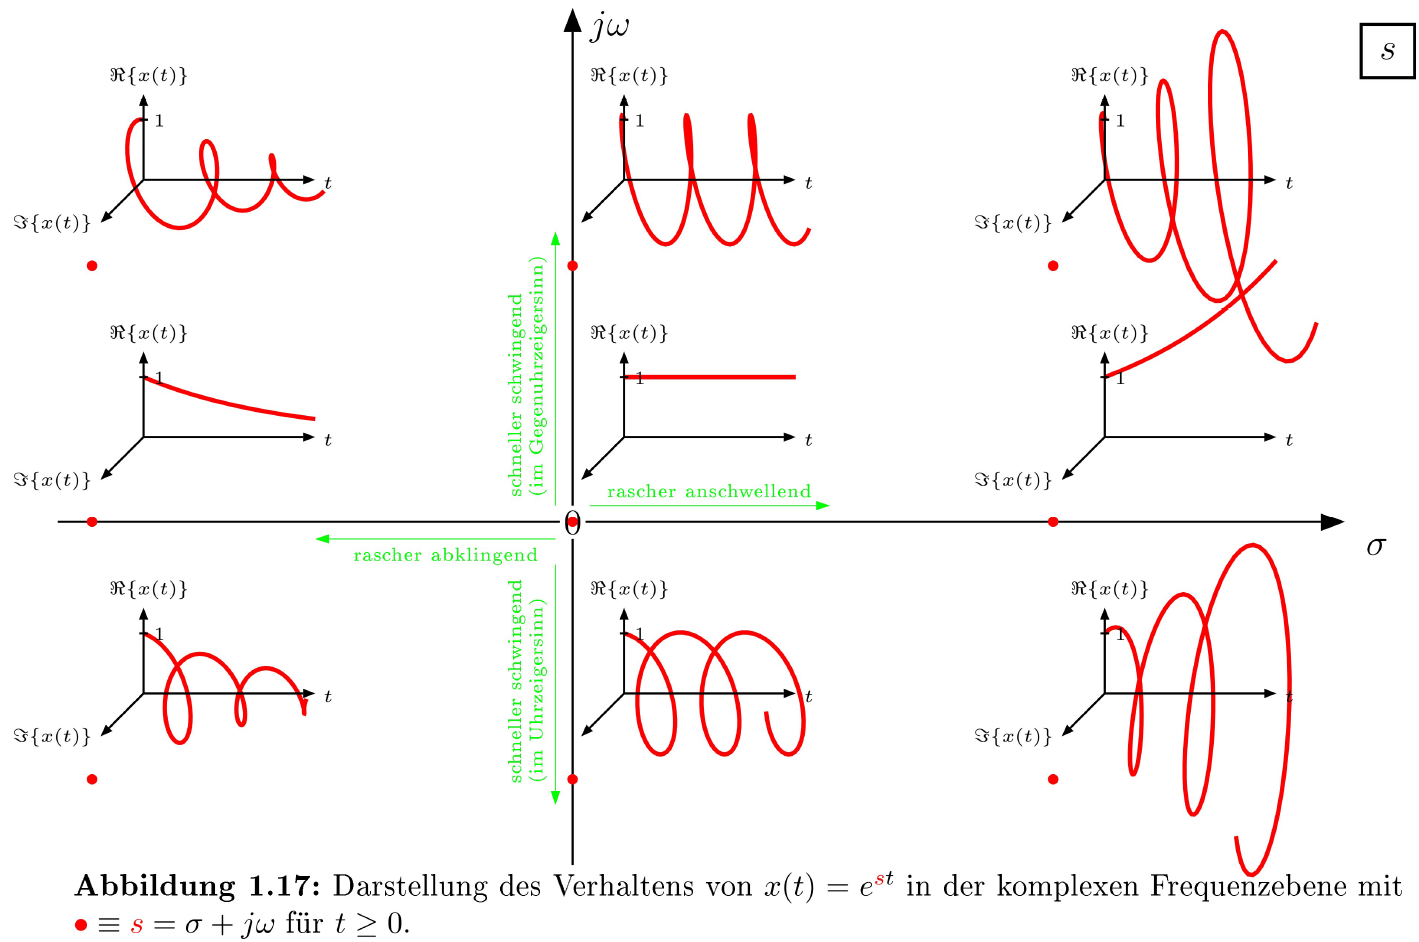
\includegraphics[width=0.88\columnwidth]{images/komplexe_frequenzen.png}
\end{center}

